%%
%% Author: thompson
%% 26.10.17
%%

% Preamble
\documentclass[11pt]{article}

% Packages
\usepackage{a4wide}
\usepackage[utf8]{inputenc}
\usepackage[ngerman]{babel}
\usepackage{scrextend}      % Intending
\usepackage{graphicx}

% Document
\begin{document}

\section{ISO-OSI Referenzmodel}
    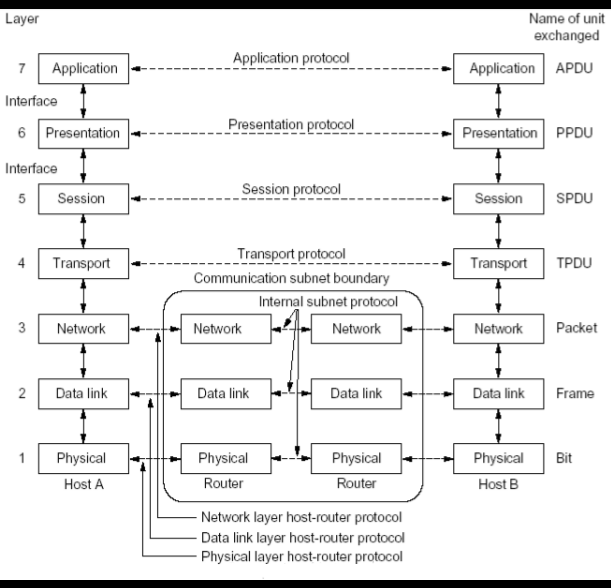
\includegraphics[width=\textwidth]{ISO_OSIReferenceModel.png}

    Das ISO-OSI Referenzmodell besteht aus verschiedenen Anwendungsschichten:
    \begin{enumerate}
        \item \textbf{\underline{Physical Layer}}\\
        Dieser Layer beschreibt die fundamentale Netzwerkkommunikation. Datentransfer via
        physischem Layer sind reine Bitstreams.

        \emph{Hardware}:
        \begin{addmargin}[1em]{1em}
            PHY-Chip: Ein PHY implementiert die Funktionen Senden und Empfangen von Daten zwischen
            Geräten mithilfe des Datalink Layers (MAC, LLC). Es enkodiert und dekodiert einkommende
            Übertragungen und  ermöglicht Galvanische Trennung (blocken ungewollter Daten).
        \end{addmargin}

        \emph{Protokolle}:
        \begin{addmargin}[1em]{1em}
            Integrated Services Digital Network: Internationaler Standard für Datenübertragung \& Telefonie\\
            Universal Serial Bus: Bussystem von Verbindungen um Daten zu übertragen\\
            Bluetooth, Ethernet, ...
        \end{addmargin}

        Grundsätzlich wird alles Hardwaretechnische über diese Schicht definiert - Kein Anschluss zum Router,
        eine unterbrochene Kabelverbindung, u.s.w..

        \item \textbf{\underline{Data Link Layer}}\\
        Der Datenlink nutzt Frames zur Übertragung von Datensätzen. Frames bestehen aus einer gewissen Anzahl
        an Bit-Blöcken und einer Prüfsumme, welche die korrekte Datenflussübertragung gewährleistet.
        Fehlerbehafte Frames können anhand dieser Summe erkannt werden und der DLL kann das jeweilige Paket verwerfen
        oder sogar korrigieren.
        Im Falle des Verwerfens ist es allerdings nicht vorgesehen das jeweilige Frame neu anzufordern.

        Mithilfe der 'Data Flow Control' kann man die Dynamik der Frameübertragung steuern, etwa wie schnell
        Blöcke verschickt werden.

        \emph{Hardware}:
        \begin{addmargin}[1em]{1em} % Left & right
            Bridges \& Switches: Arbeiten via Media Access Control(MAC) oder Logical Link Control(LLC).\\
            Die MAC-Bridge schützt gegen Kollisionen via Aufteilung des Netzes in verschiedene Kollisionsdomänen, d.H.
            ein Paket geht nur in das Netz, in welchem sich der tatsächliche Empfänger befindet.\\
            Die LLC-Bridge dient der Koppelung zweier Teilnetze mithilfe verschiedener Zugriffsverfahren, wie
            Token-Passing (Tokens werden zwischen Sendern gewechselt und dementsprechend startet Datenverkehr) oder
            Carrier Sense Multiple Access/Collision Detection (CSMA/CD; Typischer Router mit x-Medien).\\
        \end{addmargin}

        \emph{Protokolle}:
        \begin{addmargin}[1em]{1em}
            HDLC - High-Level Data Link Control: Transmition of sync/async frames\\
            SDLC - Synchronous Data Link Control: Bitsynchron \& Serielle Übertragung\\
            DDCMP - Digital Data Communications Message Protocol: Point-to-Point Transfer (Sicherheit)\\
            SPB - Shortest Path Bridging: Aufbau \& Konfig. + Multipath Routing\\
        \end{addmargin}
        \emph{Normen}: IEEE, FDDI (Fiber Distributed Data Interface), ISO\\

        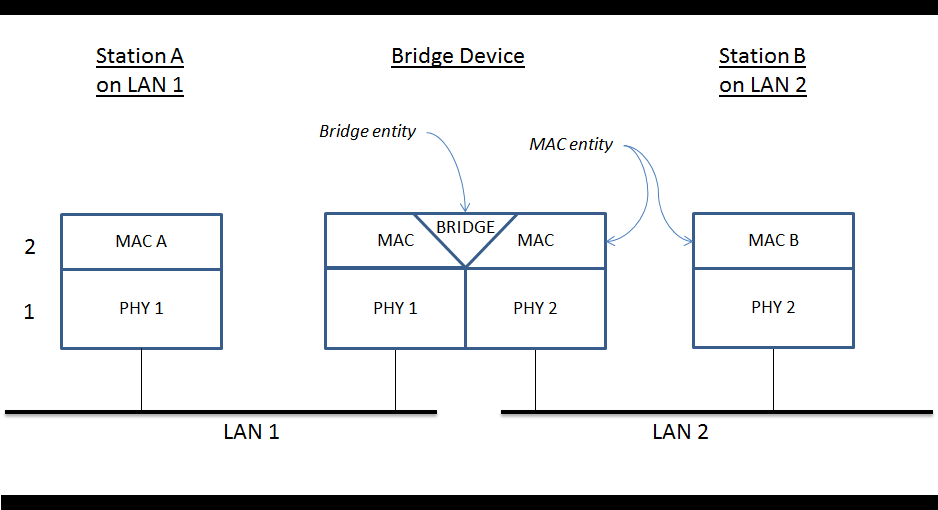
\includegraphics[width=\textwidth]{Network_Bridging.png}
        \footnote[1\small \emph{Schemata of Bridge/Switch inside a Network}]{By Crvincenzi - MS Powerpoint, CC BY-SA 3.0, https://commons.wikimedia.org/w/index.php?curid=25610536}

        \item \textbf{\underline{Network Layer}}\\
        Der "Network Layer", oder "the Routing Layer", behandelt die Weiterleitung und
        Routing durch multiple Zwischenmedien innerhalb eines Netzwerkes.

        \emph{Funktionalitäten}:
        \begin{addmargin}[1em]{1em}
            - CL-mode: Verbindungslose Kommunikation, über (TCP-)IP\\
            - Hostadressierung, jeder Host ist einzigartig identifizierbar\\
            - Weiterleitung: Partitionierung von Netzwerken in Subnetzwerke und Weiterleitung
            von Daten über Gateways und Router\\
        \end{addmargin}

        \item \textbf{\underline{Transport Layer}}\\
        Dieser beschreibt den konkreten Datentransfer von A nach B, genannt "Windowing": Wieviele Daten geschickt oder empfangen werden,
        wann Daten gesendet werden, u.s.w..

        \emph{Protokolle}:
        \begin{addmargin}[1em]{1em}
            - Transmission Control Protocol: TCP/IP - Datentransfer wird kontrolliert weitergegeben. Wird das Paket falsch oder garnicht
            empfangen, so wird eine Anfrage geschickt welche das Datenpaket neu schickt.
            Es gibt Flow- und Congestioncontrol. Grundsätzlich genutzt bei HTTP, FTP, SMTP.\\
            - User Datagram Protocol: UDP/IP - Datentransfer wird losgeschickt, ohne Kontrolle ob das Datenpaket tatsächlich ankommt.
            Es gibt also weder Flow- noch Congestioncontrol.\\
        \end{addmargin}

        \item \textbf{\underline{Session Layer}}\\
        Es beschreibt alles rund um das öffnen, schließen und managen von Sessions zwischen Usern.
        Es handelt sich dabei um einen anhaltenden Dialog der Geräte und behandelt Datensynchronisation und 'Checkpointing'\footnote[1]{Save states bei Fehler :: Laden bei Page 101 führt zu Fehler $<$=$>$  Neuladen von 1-100 nicht notwendig}.

        \emph{Protokolle}:
        \begin{addmargin}[1em]{1em}
            - ISO 8326 - OSI protocol suite: Neuverbindungsaufbau nach Störungen
            - ZIP - Zone Information Protocol (AppleTalk)
            - SMB - Server Message Block
            - RPC - Remote Procedure Call
        \end{addmargin}

        Wenn man beispielsweise eine Website aufruft, so startet der Layer eine 'Session' mit dem jeweiligen Webserver.

        \item \textbf{\underline{Presentation Layer}}\\
        Die Präsentationsschicht dient der Darstellung der Übertragenen Daten, auch 'Syntax Layer' genannt.
        Durch Konventionen wie ISO, ASCII oder EBCDIC werden die Bitcodes in erste Strukturen umgewandelt.

        Alles was im Rahmen des eigenen Betriebssystemes passiert kann dieser Schicht zugeordnet werden: Protokollkonvertierung,
        Datenübersetzung, Kompression, Enkryption, Interpretation von graphischen Kommandos,...

        \item \textbf{\underline{Application Layer}}\\
        Die Anwendungsschicht spezifiziert den Zugriff auf das Netzwerk, beispielsweise Client/Server-Verbindung, P2P, etc.

        Es stellt sicher, dass eine Applikation auf System A genauso aussieht wie auf System B, was
        prinzipiell alles wiederspiegelt womit der User direkt arbeitet, z.B. FireFox, Chrome, Skype, Outlook, ...\\

    \end{enumerate}

    Die Kommunikation derselben Schichten zwischen 2 Usern geschieht anhand der definierten Protokolle und dient grundsätzlich dem Exception-Handling:
\begin{itemize}
    \item[$\diamond$] Physical Layer: Verbindungsunterbruch auf Basis der Hardware
    \item[$\diamond$] Datalink Layer: Bitsynchrone Übertragung, Serielle Übertragung, Point2Point-Transfer, richtige MAC/LLC-Adressierung
    \item[$\diamond$] Network Layer: Verwerfen fehlerbehafteter Pakete, Routing
    \item[$\diamond$] Transport Layer: Übertragungsprotokoll: TCP-IP oder UDP-IP
    \item[$\diamond$] Session Layer: Bestätigung zum Datentransfer, Erhalt der Daten ist möglich, Verbindungsaufbau, Timeout-Handling
    \item[$\diamond$] Presentation Layer: Kodierungsformat, Enkryption, Dekryption
    \item[$\diamond$] Application Layer: Darstellung durch jeweilige User-Applikation.
\end{itemize}

    \underline{Kurzum:}\\
    - Gleiche Schichten kommunizieren mittels Protokollen miteinander\\
    - Zwischen den Schichten kommen Schnittstellen zum Einsantz\\
    - Obere Schichten bauen auf den Unteren auf.\\
    - Die 5. und 6. Schicht wird meist impliziert.\\

    \begin{addmargin}[1em]{2em}
        \textbf{\underline{Beispiel: Versenden einer E-Mail}}
    \end{addmargin}
    Das Senden einer Mail geschieht durch den User direkt im Application Layer.\\
    Dieser gibt den Datensatz weiter an den Presentation Layer, welcher die Mail in eine
    systemunabhängige Datei umschreibt, inklusive dessen Codierungsform und Enkryption.\\
    Weiter im Session Layer wird die Sitzung zum Zielempfänger spezifiziert, etwa @gmail.\\
    Der Transport Layer definiert den Datenübertragungstyp, TCP/IP, UDP/IP.\\
    Der Network Layer setzt anschließend einen Pfad fest, auf welchem das Datenpaket zum Empfänger
    gesendet wird. Dies ist später noch änderbar.\\
    Der Datalink Layer formt aus dem oben erstellten, systemunabhängigen Dateiabbild die 'Frames'.\\
    Via Bridge \& Switch wird anhand MAC/LLC die Datenübertragung kontrolliert weitergegeben.\\
    Die Physische Schicht gibt nun die Daten aus dem eigenen System einem Router, bzw. einem Bridge-Device, weiter.\\

\begin{addmargin}[1em]{0em}
    Anhand des vorgegebenen Pfades werden nun die Daten von A nach B transferiert.\\
\end{addmargin}
    In System B treffen nun die Daten aus System A via physischen Layern ein.  Der Datalinklayer setzt die Frames zusammen,
    der Network Layer bestätigt die korrekte Adressierung, der Transport Layer kommuniziert entsprechend Protokolltypes zurück,
    der Sitzungslayer bestätigt die erstellte Sitzung der Systeme. Der Presentation layer schreibt Frames in dasselbe Dateiabbild zurück
    wie vor der Transformierung in Bit und der Applikationslayer gibt die Daten dem Zieladdressaten wieder.

\end{document}